% ===================================================
% CHAPITRE 10 — LA CARELLE
% Pages imprimées 51-56 — vues 54-59
% ===================================================
\chapter{La Carelle}

% --- Page imprimée 51 — vue 54
\begin{figure}[htbp]
    \centering
    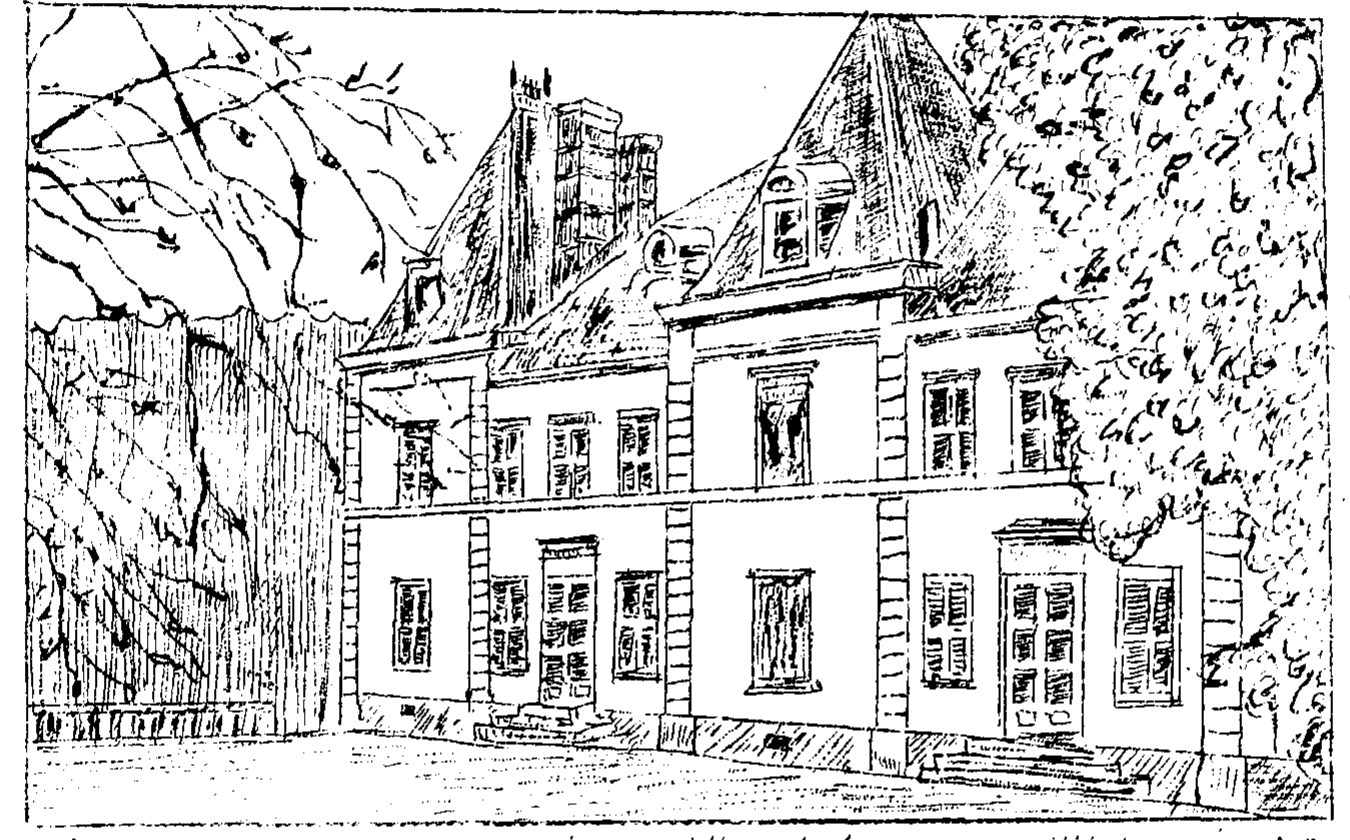
\includegraphics[width=0.72\textwidth]{Illustrations/illus-carelle-chateau.png}
    \caption*{Château de la Carelle, restauré au début de la seconde moitié du XIXème siècle.}
\end{figure}

Nous n'avons sur l'origine et les possesseurs successifs de ce fief d'autres détails que ceux donnés par l'auteur de l'histoire du Beaujolais, mieux à même que personne pour découvrir les titres concernant le château seigneurial qu'il avait reçu de ses ancêtres.

"Lacarelle, nous dit-il, était un pavillon de chasse appartenant aux Sires de Beaujeu. L'un d'eux en fit don à la famille de Nagu au XVème siècle, en récompense de ses services. Au XVIème siècle, les héritiers le vendirent à la famille Du Bost qui en céda presque tous les droits à l'église d'Ouroux où elle fonda la Chapelle de Sainte Croix".

% --- Page imprimée 52 — vue 55
Nous nous permettons ici de relever plusieurs erreurs.

Nous n'avons pas à discuter le fait de la donation rapportée par Monsieur de Lacarelle en faveur d'un membre de la famille de Nagu. Mais la date assignée par l'auteur ne peut être admise. La liste généalogique de Nagu remonte jusqu'au XIVème siècle et n'omet aucun fait saillant concernant les fiefs et les dignités. Il serait surprenant que le généalogiste ait passé sous silence un témoignage public de la reconnaissance du sire de Beaujeu en faveur de l'un des Nagu. La donation, si donation il y a, doit remonter plus haut, ou tout au moins est antérieure à l'année 1374.

Mais là où l'erreur nous paraît manifeste, c'est lorsque notre historien nous dit qu'au XVI° siècle les héritiers de Nagu vendirent le fief à la famille Du Bost. Il s'agit évidemment dans la pensée de Monsieur de Lacarelle, de Bosco, notaire à Ouroux au commencement du XVe siècle. C'est lui qui fonda en 1449 la Chapelle de Sainte-Croix. Du reste, le nom latin de Bosco se traduisit, plus tard, indifféremment par Du Bost ou Dubois. Nous l'avons trouvé déjà se rendant acquéreur d'une partie des terres de Nagu. Originaire de Beaujeu, cette famille ne put s'établir dans notre localité car Thomas de Bosco, bien que marié, mourut sans enfants.

Le fief de Lacarelle a-t-il appartenu à un Du Bost ? Tous les auteurs, se basant sur l'historien de notre province, ont répété après lui que les Du Bost, puis l'Église d'Ouroux possédèrent cette terre. Louver nous dit lui-même : "Dans l'église, il y a une chapelle de Sainte-Croix fondée par les Du Bost, à trois Messes par semaine qui a de belles rentes et un terrier". D'après ce dernier, les belles rentes et le terrier ne concernent que la chapelle ; Monsieur de Lacarelle les attribue à l'église elle-même.

L'un et l'autre, croyons-nous, sont tombés dans l'erreur ; le fief de Lacarelle n'a appartenu ni à l'église ni aux De Bosco.

Voici quelles sont nos preuves :

Thomas de Bosco restaura une ancienne chapelle dédiée à la Ste-Croix et y fonda trois Messes par semaine. Comme garantie du paiement des honoraires dus aux curés d'Ouroux, de St Mamert et d'Avenas en faveur desquels avait été faite la fondation, il hypothéqua tous les servis qui lui étaient dus sur les paroisses de Monsols, Saint
% --- Page imprimée 53 — vue 56 (suite)
Christophe, Trades, St-Mamert et les Ardillats. Dans le titre même de fondation sont énumérées les diverses reconnaissances relatées dans son terrier et les redevances de chaque tenancier.

Après cette énumération aussi complète que possible, il hypothèque encore tous les biens qu'il peut avoir dans le village d'Ouroux, au mas des Friaulx, du Clapier et de la Fosse. Les Friaulx sont près du bourg. Nous ignorons, il est vrai, l'emplacement des deux autres domaines, mais ils n'étaient pas à Lacarelle, car le terrier d'Alloignet, assez complet pour cette partie de la paroisse, eut fait mention, tout au moins de l'un de ces noms. Nous serions, du reste, porté à croire que le mas de Fosse devait être lui aussi près du bourg d'Ouroux, dans la colline de Montegouilloux ; la fontaine appelée "de la font fausse" en eut conservé le nom.

De Bosco n'ayant jamais possédé le fief de Lacarelle, ne pouvait par conséquent le céder à l'Église. Tous les documents, depuis cette époque, constatent que la Fabrique est sans ressources. Le Chapitre de Beaujeu est chargé de l'entretien du chœur et du clocher ; la nef elle-même est à la charge des paroissiens. Nous trouverions, dans le cas d'une aliénation volontaire ou forcée de ce fief de la part de notre église, quelques traces des revenus résultant de la vente.

Comment expliquer l'erreur dans laquelle sont tombés les historiens au sujet des possesseurs de ce fief ? Pour cela étudions le texte même de la fondation de Sainte-Croix. En rétablissant ce texte surchargé de fautes par le copiste, nous lisons ces mots :

"Ad remedium et salutem, etc..., pour le remède et le salut de son âme et des âmes de ses parents, de ses bienfaiteurs et de ses amis décédés, principalement de celle de son père, de sa mère et de son épouse, et de vénérable homme de Dieu d'heureuse mémoire, Jean de Lacarelle, prêtre et son parent, dont lui Thomas est, se dit et affirme être l'héritier universel..."

Comme on le voit De Bosco est héritier d'un de ses cousins prêtre Jean de Lacarelle, et cela, avec d'autant plus de raison que, comme nous le verrons plus tard, les noms de famille n'existaient généralement pas encore et qu'on se contentait d'ajouter à son nom de Baptême celui de la terre, du mas, de la paroisse qu'on habitait.

% --- Page imprimée 54 — vue 57
Ainsi Lacarelle n'était qu'un surnom adopté par le prêtre Jean et nous devrions traduire "Joannès de Carella" par Jean de Charolles ou Jean le Charolais. Dans la Charte 271 du Cartulaire d'Aymard de Cluny et qui date de l'an 950, nous lisons ces mots : "res sita in pago Augustodunensi, in agro sive in terminis de Carella, in villa Collonicas ; cette chose est située dans le pays d'Autun, l'ager ou les limites de Charolles, le village de Collonges, commune de Vendenesse". Carella était donc bien la même chose que Charolles.

Plus tard le nom de Charolles, Carelle ou Charolais se transforma par l'usage et devint le nom de plusieurs familles dont quelques-unes subsistent encore. Il est probable que l'une d'elles a donné son nom à la vallée elle-même qui, jusqu'au XVe siècle, fut désignée sous le nom de Combe d'Aissard. Le terrier de Vauxrenard (1459) énumère les servis dus par Claude fils de Martin Colonjean alias de Carella "Surnommé de Lacarelle" à cause des biens qu'il possède aux Essarts, servis dus au prieuré de ladite paroisse et qui s'élèvent à 6 sols 7 deniers viennois, 6 deniers tournois, 2 ras et demi d'avoine. En 1520, le terrier d'Alloignet mentionne le mas de Lacarelle dans une reconnaissance faite par Claude de Lacarelle. Cette famille s'est éteinte dans le siècle suivant, au château du Sauzay. Le mas qu'elle posséda prit, vers cette époque, et garda définitivement le nom de la famille, comme cela est arrivé fréquemment à Ouroux, par exemple à Deguin, les Pourchoux, les Jambons, etc.

Il nous semble donc acquis que le fief de Lacarelle n'a jamais appartenu ni aux Dubost, ni à l'Église. Une lecture superficielle de l'acte de fondation de la Chapelle de Sainte-Croix a pu seule induire en erreur ceux qui se sont occupés de notre histoire locale.

Les Carrige ont donc dû acquérir directement des Nagu eux-mêmes la terre de Lacarelle au moment où ils vendaient le fief d'Arcis, c'est-à-dire au commencement du XVIe siècle. La date fournie par cette hypothèse s'accorderait avec celle donnée par Monsieur de Lacarelle.

% --- Page imprimée 55 — vue 58
L'histoire, du reste, semble confirmer cette conclusion. Le 20 Avril 1526, Charles de Bourbon céda à Hugues de Nagu la « justice haute, basse et moyenne de Quincié et Marchampt pour l'indemniser des démolitions de ses maisons et châteaux, dommages et intérêts par lui et les siens soufferts et aussi en considération des services à lui faits ».

Pourquoi ces démolitions ? Quels en furent les auteurs ? Très probablement les troupes qui vinrent s'établir en garnison dans le Beaujolais après la trahison du connétable.

La famille des Carrige occupa, dans notre région, une situation honorable. Les seuls noms qui nous aient été conservés se lisent dans la liste des dignitaires du Chapitre de Beaujeu. Antoine, en 1606, Philibert en 1617, François en 1655 sont élus Chantres de Notre-Dame.

Vers la fin du même siècle nous retrouvons le nom de Carrige associé à celui de De Lafont et de MAGNIN-VERTPRÉ. Honoré de Lafont a pour femme Jeanne Carrige qui mourut le 7 Janvier 1725.

En 1610, par suite d'alliance, Lacarelle passa dans la famille de Magnin-Vertpré. Les MAGNIN avaient ajouté à leur nom celui de la Seigneurie de Vertpré en Lyonnais ; ils possédaient également le fief de Pierreux à Odenas.

Au mois de Janvier 1639, le château devint la proie des flammes, la famille de Magnin perdit tous ses titres dans l'incendie. Une enquête eut lieu à ce sujet le 15 Juillet 1645 pour établir par témoignage l'ancienneté de sa noblesse et suppléer aux titres brûlés.

Jehan Magnin, écuyer, est qualifié en 1647 de Seigneur de Ponchon et Lacarelle. En 1678, Jean Marie prend le titre de seigneur de Vertpré, Ponchon et Lacarelle. Il épouse Marie Carrige comme nous le prouve un acte de Baptême, en 1688. Elle signe comme marraine en 1700, et nous a conservé le nom d'une de ses filles Bénigne de Vertpré.

Nous ne saurions passer sous silence le seul fait saillant qui concerne Jean-Marie Magnin et nous donne une idée des mœurs de l'époque. Il nous suffira de donner le texte même du document :

« À la requête de Joseph Philibert de Thibault seigneur Despré, Le Terreau, Chevagny, Le Lombard et autres places et Jean-Marie Magnin, sieur de Vertpré soit remontré à Jean Maillard soit disant bourgeois de Lion qu'ils ont été obligés de faire informer par devant le sieur juge de Beaujeu contre ledit Maillard non seulement pour raison des
% --- Page imprimée 56 — vue 59 (suite)
injures atroces proférées par ledit Mallard, mais à cause des exécrables jurements et blasphèmes qu'il aurait faits de propos délibéré du Saint nom de Dieu publiquement en pleine rue de Beaujeu, au vu et scandale du public... etc,..". Ceci se passait en 1680.

Le 17 Octobre 1717, Jean de Magnin, écuyer, seigneur de Pierreux, ayant épousé Marie Marguerite de la Roche, une discussion judiciaire s'éleva sur la quotité des droits auxquels la dite dame avait à prétendre. Un arrangement s'en suivit qui amena un échange de propriétés et par contrat du 5 Octobre 1719, le fief de Lacarelle fut cédé à Joseph de la Roche, écuyer, seigneur de Nully, frère de Marie Marguerite. Le 15 mars 1721, il prêta foi et hommage entre les mains du duc d'Orléans, sire et baron du Beaujolais, pour sa terre et seigneurie de Lacarelle. Ses descendants la possédèrent jusqu'en 1860, époque à laquelle Monsieur Sosthène de Lacarelle la vendit à Monsieur Bourgeot, banquier à Villefranche.

Mr Bourgeot fit restaurer le château par Louis Bresson, l'éminent architecte lyonnais. "Le centre du château est occupé par un hall à deux étages, éclairé par le haut et soutenu par des colonnades de style pompéien du plus charmant effet. Tout autour s'ouvrent les salons, salle de billard, salle à manger, etc. et tout cela garni, tapissé, bondé dans un ordre merveilleux et avec un goût exquis de vieux meubles, d'armures, de statues, de tableaux : un véritable musée dont chaque pièce a été choisie une à une par un chercheur passionné pour le beau et classée par un amateur amoureux de l'antiquité".

La fille et le gendre de Mme Vve Bourgeot, Mme et Mr Riboud héritèrent ce beau château et le domaine de La Carelle.

% --- Recadrages directs de la vue originale : chaque bloc contient
% --- le blason, son nom manuscrit et son descriptif manuscrit.
\noindent
\begin{minipage}[t]{0.31\textwidth}
    \centering
    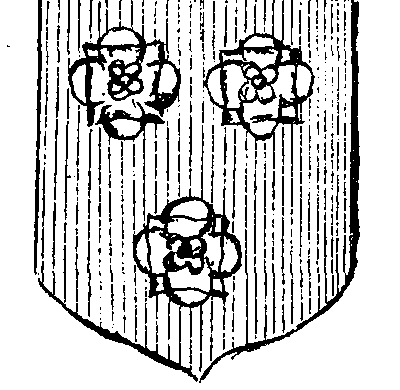
\includegraphics[height=0.20\textheight,keepaspectratio]{Illustrations/illus-carelle-carrige.png}
\end{minipage}\hfill
\begin{minipage}[t]{0.31\textwidth}
    \centering
    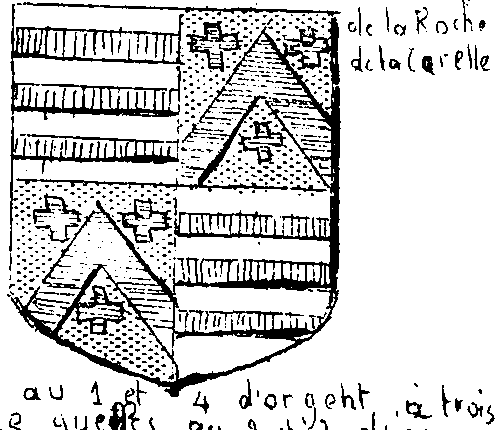
\includegraphics[height=0.20\textheight,keepaspectratio]{Illustrations/illus-carelle-roche.png}
\end{minipage}\hfill
\begin{minipage}[t]{0.31\textwidth}
    \centering
    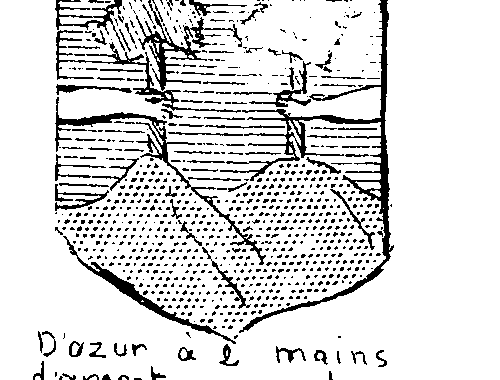
\includegraphics[height=0.20\textheight,keepaspectratio]{Illustrations/illus-carelle-magnin.png}
\end{minipage}
